\documentclass{beamer}
\setbeamertemplate{navigation symbols}{}
\usepackage{beamerthemeshadow}


\begin{document}

\title{Active Learning}  
\author{Kacper Sokol}
\date{\today} 
\begin{frame}
\titlepage
\end{frame}




\begin{frame}
  \frametitle{Table of contents}
  \tableofcontents
\end{frame} 


\section{Concept of learning} 
  \subsection{Clustering}
  \begin{frame}%[plain]
    \frametitle{Find two clusters} 
    \begin{figure}
      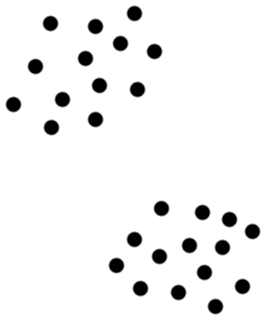
\includegraphics[scale=.5]{graphics/presentation/clusters1} 
    \end{figure}
  \end{frame}

  \begin{frame}%[plain]
    \frametitle{Find two clusters cont.} 
    \begin{figure}
      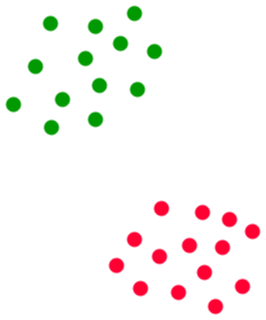
\includegraphics[scale=.5]{graphics/presentation/clusters1a} 
    \end{figure}
  \end{frame}

  \begin{frame}%[plain]
    \frametitle{Find two clusters cont.} 
    \begin{figure}
      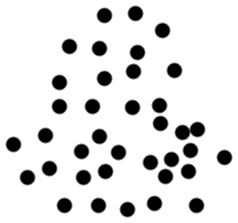
\includegraphics[scale=.5]{graphics/presentation/clusters2} 
    \end{figure}
  \end{frame}

  \begin{frame}%[plain]
    \frametitle{Find two clusters cont.} 
    \begin{figure}
      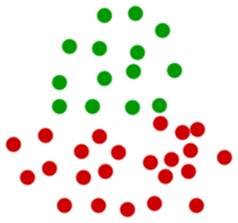
\includegraphics[scale=.5]{graphics/presentation/clusters2a} 
    \end{figure}
  \end{frame}

  \begin{frame}%[plain]
    \frametitle{Find two clusters cont.} 
    \begin{figure}
      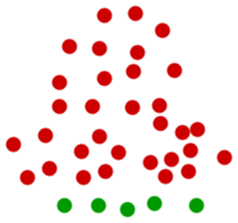
\includegraphics[scale=.5]{graphics/presentation/clusters2b} 
    \end{figure}
  \end{frame}

  \begin{frame}%[plain]
    \frametitle{Find two clusters cont.} 
    \begin{figure}
      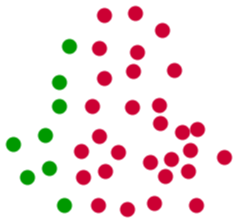
\includegraphics[scale=.5]{graphics/presentation/clusters2c} 
    \end{figure}
  \end{frame}

  \begin{frame}%[plain]
    \frametitle{Find two clusters cont.} 
    \begin{figure}
      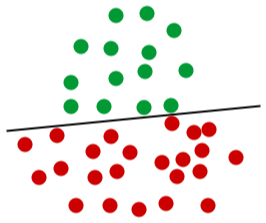
\includegraphics[scale=.5]{graphics/presentation/clusters2d} 
    \end{figure}
  \end{frame}

\subsection{The task}
  \begin{frame}
    \frametitle{Linear classifier}
    \begin{columns}
      \begin{column}{5cm}
        \begin{itemize}
          \item We are handling \textbf{binary classification}.
          \item The data are \textbf{linearly separable}.
          \item Therefore, our goal is to find two clouds of points separated by a straight line and make no error in separation.
        \end{itemize}
      \end{column}
      \begin{column}{5cm}
        \begin{figure}
          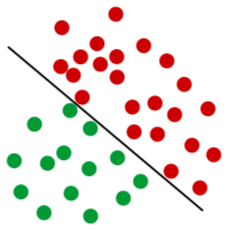
\includegraphics[scale=.4]{graphics/presentation/clusters2e} 
        \end{figure}
        \begin{itemize}
          \item green---a bike; red---a car
          \item x-axis---age of a person
          \item y-axis---distance form home to office/school
        \end{itemize}
      \end{column}
    \end{columns}
  \end{frame}

  \begin{frame}
    \frametitle{Linear classifier}
  \end{frame}

  \begin{frame}
    \frametitle{Supervised learning}
  \end{frame}

\subsection{Active learning}
  \begin{frame}
    \frametitle{Naive active learning}
  \end{frame}

  \begin{frame}
    \frametitle{Slightly better active learning}
  \end{frame}

  \begin{frame}
    \frametitle{Perfect active learning}
  \end{frame}


\section{Is it really exploration vs. exploitation?} 
\subsection{Multi-armed bandits as a workhorse}
  \begin{frame}
  \frametitle{MAB}
  \end{frame}

  \begin{frame}
  \frametitle{Ingredients of active learning}
  \end{frame}

  \begin{frame}
  \frametitle{Applying MAB to active learning}
  \end{frame}
\subsection{The experiment}
  \begin{frame}
  \frametitle{The dataset}
  \end{frame}
  \begin{frame}
  \frametitle{Arriving at optimal classifier}
  \end{frame}

\end{document}

%%%%%%%%%%%%%%%%%%%%%%%%%%%%%%%%%%%%%%%%%%%%%%%%%%%%%%%%%%%%%%%%%%%%%%%%%%%%%%%%
% \begin{block}{title of the bloc}
% bloc text
% \end{block}
%
% \begin{exampleblock}{title of the bloc}
% bloc text
% \end{exampleblock}
%
% \begin{alertblock}{title of the bloc}
% bloc text
% \end{alertblock}
% 
% 
% \pause 
% 
% \begin{itemize}
% \item<1-> subject 1
% \item<3-> subject 2
% \item<5-> subject 3
% \end{itemize}
% 
% 
% \begin{overprint}
% \includegraphics<2>{PIC1}
% \includegraphics<4>{PIC2}
% \includegraphics<6>{PIC3}
% \end{overprint}
%%%%%%%%%%%%%%%%%%%%%%%%%%%%%%%%%%%%%%%%%%%%%%%%%%%%%%%%%%%%%%%%%%%%%%%%%%%%%%%%
